\documentclass[aspectratio=169,10pt]{beamer}
\usetheme[
%%% options passed to the outer theme
%    progressstyle=movCircCnt,   %either fixedCircCnt, movCircCnt, or corner
%    rotationcw,          % change the rotation direction from counter-clockwise to clockwise
%    shownavsym          % show the navigation symbols
  ]{AAUsimple}
  
% If you want to change the colors of the various elements in the theme, edit and uncomment the following lines
% Change the bar and sidebar colors:
%\setbeamercolor{AAUsimple}{fg=yellow!20,bg=yellow}
%\setbeamercolor{sidebar}{bg=red!20}
% Change the color of the structural elements:
%\setbeamercolor{structure}{fg=red}
% Change the frame title text color:
%\setbeamercolor{frametitle}{fg=blue}
% Change the normal text color background:
%\setbeamercolor{normal text}{fg=black,bg=gray!10}
% ... and you can of course change a lot more - see the beamer user manual.

\usepackage[utf8]{inputenc}
\usepackage[english]{babel}
\usepackage[T1]{fontenc}
% Or whatever. Note that the encoding and the font should match. If T1
% does not look nice, try deleting the line with the fontenc.
\usepackage{helvet}
\usepackage{pgffor}

% Pseudocode
\usepackage{xcolor}
\usepackage[linesnumbered,ruled,vlined]{algorithm2e}

% subfigure
\usepackage{subcaption}

% draw figures
\usepackage{tikz}
\usetikzlibrary{arrows}

% Highligthing
\newcommand{\hl}[1]{%
  \begin{center}
    \colorbox{yellow}{#1}
  \end{center}
}

% Layout
\setlength{\parskip}{1em}

% colored hyperlinks
\newcommand{\chref}[2]{%
  \href{#1}{{\usebeamercolor[bg]{AAUsimple}#2}}%
}

\title{Data Mining Exam}

% \subtitle{}  % could also be a conference name

\date{\today}

\author{
  Kasper Rosenkrands
}

% - Give the names in the same order as they appear in the paper.
% - Use the \inst{?} command only if the authors have different
%   affiliation. See the beamer manual for an example

\institute[
%  {\includegraphics[scale=0.2]{aau_segl}}\\ %insert a company, department or university logo
  % Audio Analysis Lab, CREATE\\
  % Aalborg University\\
  % Denmark
] % optional - is placed in the bottom of the sidebar on every slide
{% is placed on the bottom of the title page
  %Department of Mathematical Sciences\\
  Aalborg University\\
  Denmark
  
  %there must be an empty line above this line - otherwise some unwanted space is added between the university and the country (I do not know why;( )
}

% specify a logo on the titlepage (you can specify additional logos an include them in 
% institute command below
\pgfdeclareimage[height=1.5cm]{titlepagelogo}{AAUgraphics/aau_logo_new} % placed on the title page
%\pgfdeclareimage[height=1.5cm]{titlepagelogo2}{AAUgraphics/aau_logo_new} % placed on the title page
\titlegraphic{% is placed on the bottom of the title page
  \pgfuseimage{titlepagelogo}
%  \hspace{1cm}\pgfuseimage{titlepagelogo2}
}

\begin{document}
% the titlepage
{\aauwavesbg%
\begin{frame}[plain,noframenumbering] % the plain option removes the header from the title page
  \titlepage
\end{frame}}
%%%%%%%%%%%%%%%%

% TOC
% \begin{frame}{Agenda}{}
% \tableofcontents
% \end{frame}
%%%%%%%%%%%%%%%%

\section{Clustering}

% \subsection{Overview}
% \begin{frame}{\secname}{\subsecname}
%   \begin{itemize}
%     \item What is clustering?
%     \item K-Means optimization problem and algorithm
%     \item Implementation of the K-Means algorithm and an example
%     \item Hierarchical Clustering (briefly)
%   \end{itemize}
% \end{frame}

\subsection{Introduction}
\begin{frame}{\secname}{\subsecname}
  \textbf{Clustering} is a way to categorize data to impose structure.
  
  A use case is recommender systems (Amazon, Spotify, Netflix), where a user is recommended items that bought/listened to/watched by other users with similar interests.
\end{frame}

\subsection{K-Means Optimization Problem}
\begin{frame}{\secname}{\subsecname}
  % \begin{itemize}
  %   \item One example of a clustering algorithm is \textbf{K-Means}
  % \end{itemize}
  Given $D = (x_1, \ldots, x_n)$ where $x_i \in \mathbb{R}^p$, $K \in \mathbb{N}$ and let $C_1, \ldots, C_K$ denote different groups of the $x_i$'s.
  
  The K-Means algorithm tries to solve
  \begin{align}
    \min_{C_1, \ldots, C_K} \left\{\sum_{k=1}^K W(C_k)\right\}, \label{k-means-general-problem}
  \end{align}
  where $W(C_k)$ denotes the \textbf{within cluster variation}, in other words the dissimilarity of the group.
  \vspace{10pt}
  
  {\small The most common dissimilarity measure is the is the squared Euclidean distance
  \begin{align}
    W(C_k) := \frac{1}{|C_k|} \sum_{i,i' \in C_k} \sum_{j = 1}^p (x_{i,j} - x_{i',j})^2.
  \end{align}}
\end{frame}

\begin{frame}{\secname}{\subsecname}
  If we by $\bar{x}_{k,j} = \frac{1}{|C_k|}\sum_{i \in C_k} x_{i,j}$ denote the mean value of the $j$'th dimension in cluster $k$, it can be shown that
  \begin{align}
    \frac{1}{|C_k|} \sum_{i,i' \in C_k} \sum_{j = 1}^p (x_{i,j} - x_{i',j})^2 = 2 \sum_{i \in C_k} \sum_{j = 1}^p (x_{i,j} - \bar{x}_{k,j})^2.
  \end{align}
  If we further note that $\bar{x}_{k,j} = \min_{\mu_k} \left\{ \sum_{i \in C_k} \sum_{j = 1}^p (x_{i,j} - \mu_k)^2\right\}$ this implies that the optimization problem in \eqref{k-means-general-problem} can be rewritten as
  \begin{align}
    \min_{C_1, \ldots, C_k, \mu_1, \ldots, \mu_k} \left\{ \sum_{k = 1}^K \sum_{i \in C_k} \sum_{j = 1}^p (x_{i,j} - \mu_k)^2 \right\}.
  \end{align}
\end{frame}

\subsection{K-Means Algorithm}
\begin{frame}{\secname}{\subsecname}
  The K-Means algorithm is now able to exploit the new formulation of the optimization problem and iteratively solve for $\{C_1, \ldots, C_k\}$ and $\{\mu_1, \ldots, \mu_k\}$.

  This makes K-Means a greedy algorithm because, in each iteration it chooses optimal values for $\{C_1, \ldots, C_k\}$ and $\{\mu_1, \ldots, \mu_k\}$.

  Convergence of the algorithm is therefore ensured, however we cannot guarantee it will find the global optimum.
\end{frame}

\begin{frame}{\secname}{\subsecname}
  \begingroup
  \footnotesize
  \begin{algorithm}[H]
    \DontPrintSemicolon
    Assign each obsevation to a cluster randomly\;
    \ForEach{Cluster}{Compute the centroid\;}
    \ForEach{Observation}{
        Compute distance to all centroids\;
        Assign to the closest \;
    }
    \While{Centroids have not changed since last iteration}{
      \ForEach{Observation}{
        Compute distance to all centroids\;
        Assign to the closest \;
      }
      \ForEach{Cluster}{
        Compute the centroid\;
      }
    }
    \Return{Clusters}
    \caption{K-Means}
  \end{algorithm}
  \endgroup
\end{frame}

\subsection{Implementation of K-Means}
% \begin{frame}{\secname}{\subsecname}
% % my_kmeans <- function(data, K, animate = F, size = 3) {
% %   data$cluster <- as.factor(sample(c(1:K), size = nrow(data), replace = T))
% %   initial_cents <- calculate_cents(data, K)
  
% %   data_list <- list()
% %   data_list[[1]] <- data
% %   data_list[[2]] <- update_cluster(data, initial_cents)
  
% %   i = 1
% %   while (!identical(data_list[[i]]$cluster, data_list[[i + 1]]$cluster)) {
% %     cents <- calculate_cents(data_list[[i + 1]], K)
% %     data_list[[i + 2]] <- update_cluster(data_list[[i + 1]], cents)
% %     i = i + 1
% %   }
  
% %   cents <- calculate_cents(data_list[[i + 1]], K)
% % }
% \end{frame}

\subsection{An example of the K-Means algorithm}
\foreach \nn in{01,02,03,04,05,06,07,08,09,10,11,12,13}{
\begin{frame}{\secname}{\subsecname}
  \begin{figure}  
    \centering
    \includegraphics[width=.6\textheight]{scripts/kmeans-animation/animation_page_00\nn.png}
    \caption{Iteration \nn}
  \end{figure}
\end{frame}
}

\subsection{Number of clusters}
\begin{frame}{\secname}{\subsecname}
  Prior to running K-Means we need to determine the number of clusters.
  For some use cases this number may be predetermined by external factors.
  If the number of clusters is not predetermined, the data itself can indicate the optimal number.

  The \textbf{total sum of squares} (total variance in the data) and the \textbf{within cluster sum of squares} are given by
  \begin{align*}
      {\color{teal}SS_{total} = \sum_{i=1}^n (x_i - \Bar{x})^2, \quad \Bar{x} = \frac{1}{n} \sum_{i = 1}^n x_i,} \quad {\color{violet}SS_{W_k} = \sum_{i \in C_k} (x_i - \Bar{x}_k)^2, \quad \Bar{x}_k = \frac{1}{n_k}\sum_{i \in C_k} x_i.}
  \end{align*}
  Then the \textbf{total within sum of squares} becomes $SS_{W} = \sum_{k=1}^K SS_{W_k}$.
  Using this we can calculate the \textbf{percentage of variance explained} as $PVE = SS_W/SS_{total}$.
\end{frame}

\begin{frame}{\secname}{\subsecname}
  We can then use what is called the \textbf{elbow method} to determine  number of clusters.
  \begin{figure}
    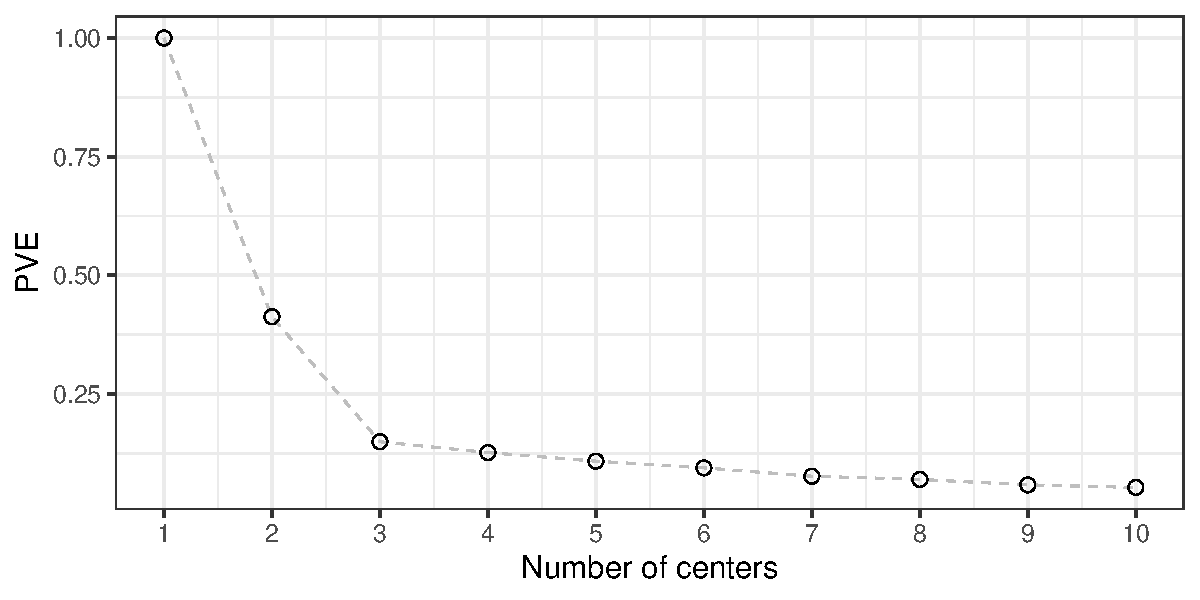
\includegraphics[width=.65\textwidth]{scripts/output/scree_plot.pdf}
    \caption{Scree plot showing the number of clusters against percentage of variance explained.}
  \end{figure}
\end{frame}

\subsection{Hierarchical Clustering}
\begin{frame}{\secname}{\subsecname}
  \begin{columns}
    \begin{column}{.7\textwidth}  
      Hierarchical clustering is a method which seeks to build a hierarchy of clusters.
      
      In general there are two approaches to obtain this hierarchy, starting from the bottom or from the top (so to speak):
      \begin{enumerate}
        \item \textbf{Agglomerative}: This is the bottom up approach, it starts by having each observation in its own cluster and then it merges the most similar together.
        \item \textbf{Divise}: This is the top down approach, it start by putting all observations in one cluster and then splits recursively to obtain more and more homogenous clusters.
      \end{enumerate}
    \end{column}
    \begin{column}{.3\textwidth}
      \resizebox{\textwidth}{!}{
        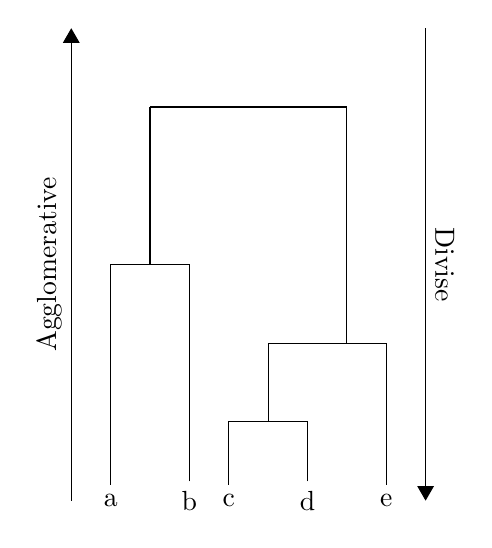
\begin{tikzpicture}[sloped]
          \node (a) at (-2,0) {a};
          \node (b) at (-1,0) {b};
          \node (c) at (-0.5,0) {c};
          \node (d) at (0.5,0) {d};
          \node (e) at (1.5,0) {e};
          \node (ab) at (-1.5,3) {};
          \node (cd) at (0,1) {};
          \node (cde) at (1,2) {};
          \node (all) at (-1.5,5) {};
          
          \draw  (a) |- (ab.center);
          \draw  (b) |- (ab.center);
          \draw  (c) |- (cd.center);
          \draw  (d) |- (cd.center);
          \draw  (e) |- (cde.center);
          \draw  (cd.center) |- (cde.center);
          \draw  (ab.center) |- (all.center);
          \draw  (cde.center) |- (all.center);
          
          \draw[->,-triangle 60] (-2.5,0) -- node[above]{Agglomerative} (-2.5,6);
          \draw[->,-triangle 60] (2,6) -- node[above]{Divise} (2,0);
        \end{tikzpicture}
      }
    \end{column}
  \end{columns}
\end{frame}

\subsection{Linkages}
\begin{frame}{\secname}{\subsecname}
  In order to quantify the similarity between observations we need to establish a dissimilarity measure.
  However there are many ways to define dissimilarity, or linkage, between groups of observations.

  \begin{enumerate}
    \item \textbf{Single}: The smallest pairwise dissimilarity.
    \item \textbf{Complete}: The largest pairwise dissimilarity.
    \item \textbf{Average}: The average dissimilarity between observations.
    \item \textbf{Centroid}: The dissimilarity between centroids of clusters.\footnote{Squared distance can cause inversions as we ``create'' new data points.}
  \end{enumerate}

  Another consideration is what distance measure to use, typically the Euclidean distance is used, but for other use cases one might opt for the Manhattan distance etc.
\end{frame}

\begin{frame}{\secname}{\subsecname}
  \begin{figure}
    \centering
    \begin{subfigure}[t]{.45\textwidth}
      \centering
      \resizebox{.9\textwidth}{!}{
        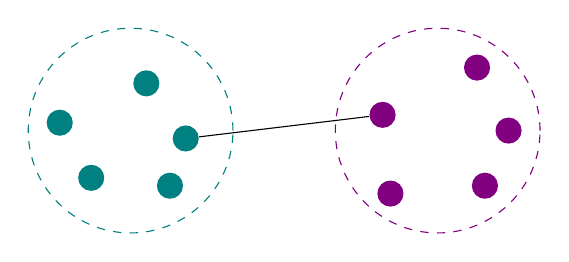
\begin{tikzpicture}
          \foreach \x\y [count=\xi from 1] in {1.7/0.9, 0.1/1.1, 0.5/0.4, 1.5/0.3, 1.2/1.6}{%
            \node[circle, color=black, fill=teal, minimum size=3pt] (\xi) at (\x, \y) {};
          }
          \foreach \x\y [count=\xi from 11] in {1.8/1, 0.2/1.2, 0.3/0.2, 1.5/0.3, 1.4/1.8}{%
            \node[circle, color=black, fill=violet, minimum size=3pt] (\xi) at (\x+4, \y) {};
          }

          \draw [dashed, color=teal] (1,1) ellipse (1.3cm and 1.3cm);
          \draw [dashed, color=violet] (1+4-.1,1) ellipse (1.3cm and 1.3cm);

          \draw (1) -- (12);
        \end{tikzpicture}
      }
      \caption{Single.}
    \end{subfigure}\hfill
    \begin{subfigure}[t]{.45\textwidth}
      \centering
      \resizebox{.9\textwidth}{!}{
        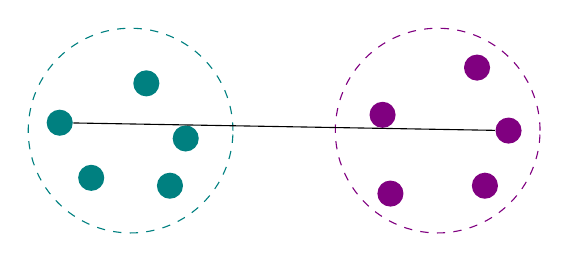
\begin{tikzpicture}
          \foreach \x\y [count=\xi from 1] in {1.7/0.9, 0.1/1.1, 0.5/0.4, 1.5/0.3, 1.2/1.6}{%
            \node[circle, color=black, fill=teal, minimum size=3pt] (\xi) at (\x, \y) {};
          }
          \foreach \x\y [count=\xi from 11] in {1.8/1, 0.2/1.2, 0.3/0.2, 1.5/0.3, 1.4/1.8}{%
            \node[circle, color=black, fill=violet, minimum size=3pt] (\xi) at (\x+4, \y) {};
          }

          \draw [dashed, color=teal] (1,1) ellipse (1.3cm and 1.3cm);
          \draw [dashed, color=violet] (1+4-.1,1) ellipse (1.3cm and 1.3cm);

          \draw (2) -- (11);
        \end{tikzpicture}
      }
      \caption{Complete.}
    \end{subfigure}\hfill
    \begin{subfigure}[t]{.45\textwidth}
      \centering
      \resizebox{.9\textwidth}{!}{
        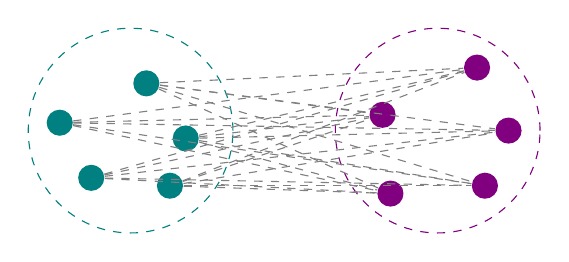
\begin{tikzpicture}
          \foreach \x\y [count=\xi from 1] in {1.7/0.9, 0.1/1.1, 0.5/0.4, 1.5/0.3, 1.2/1.6}{%
            \node[circle, color=black, fill=teal, minimum size=3pt] (\xi) at (\x, \y) {};
          }
          \foreach \x\y [count=\xi from 11] in {1.8/1, 0.2/1.2, 0.3/0.2, 1.5/0.3, 1.4/1.8}{%
            \node[circle, color=black, fill=violet, minimum size=3pt] (\xi) at (\x+4, \y) {};
          }

          \draw [dashed, color=teal] (1,1) ellipse (1.3cm and 1.3cm);
          \draw [dashed, color=violet] (1+4-.1,1) ellipse (1.3cm and 1.3cm);

          \foreach \x in {1,...,5}{
            \foreach \y in {11,...,15}{
              \draw[dashed, color=gray] (\x) -- (\y);
            }
          }
        \end{tikzpicture}
      }
      \caption{Average.}
    \end{subfigure}\hfill
    \begin{subfigure}[t]{.45\textwidth}
      \centering
      \resizebox{.9\textwidth}{!}{
        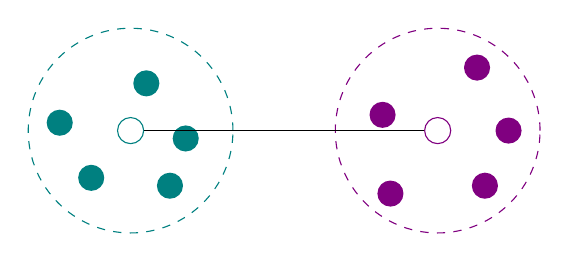
\begin{tikzpicture}
          \foreach \x\y [count=\xi from 1] in {1.7/0.9, 0.1/1.1, 0.5/0.4, 1.5/0.3, 1.2/1.6}{%
            \node[circle, color=black, fill=teal, minimum size=3pt] (\xi) at (\x, \y) {};
          }
          \foreach \x\y [count=\xi from 11] in {1.8/1, 0.2/1.2, 0.3/0.2, 1.5/0.3, 1.4/1.8}{%
            \node[circle, color=black, fill=violet, minimum size=3pt] (\xi) at (\x+4, \y) {};
          }

          \draw [dashed, color=teal] (1,1) ellipse (1.3cm and 1.3cm);
          \draw [dashed, color=violet] (1+4-.1,1) ellipse (1.3cm and 1.3cm);

          \node[draw, circle, color=teal, minimum size=3pt] (cent1) at (1, 1) {};
          \node[draw, circle, color=violet, minimum size=3pt] (cent2) at (1+4-.1,1) {};

          \draw (cent1) -- (cent2);
        \end{tikzpicture}
      }
      \caption{Centroid.}
    \end{subfigure}
    \caption{The 4 different types of linkages presented on the slide before.}
  \end{figure}
\end{frame}

\begin{frame}{\secname}{\subsecname}
  
\end{frame}

\section{Shrinkage}

% \subsection{Overview}
% \begin{frame}{\secname}{\subsecname}
%   \hl{Write theory about ridge, lasso and elastic net - including coordinate descent etc.}
%   \hl{Find an example to compare the 3 methods on}
% \end{frame}

\subsection{Variable Selection and Regularization}
\begin{frame}{\secname}{\subsecname}
  Because it is often cheaper to obtain multiple observations from a few samples than to obtain more samples, thus increasing the number of explanatory variables in a regression model, a linear regression model would be prone to increasing variance.
  
  When extending linear regression to multiple exaplanatory variables the main objectives is:
  \begin{itemize}
    \item \textbf{Model Interpretability}: Models with fewer variables are often more easy to interpret results from and are therefore better to use for decision making.
    \item \textbf{Predition Accuracy}: If by introducing some bias we are able to dramatically improve prediction accuracy, this would be worth considering (bias-variance tradeoff).
  \end{itemize}
\end{frame}

\begin{frame}{\secname}{\subsecname}
  There are multiple tools we can use in this pursuit
    \begin{itemize}
      \item \textbf{Subset Selection}: Works by fitting lots of models with different combinations of predictors. Then we can find out which variables are most related to the response and we can select these.
      \item \textbf{Dimensionality Reduction}: Works by projecting explanatory variables into a smaller dimensional space and use these projections as predictors.
      \item \textbf{Shrinkage Methods}: Works by fitting a model using all predictors while shrinking coefficients towards zero, to reduce variance. Some shrinkage methods can also perform variable selection by shrinking coefficients to exactly zero. 
    \end{itemize}
\end{frame}

\begin{frame}{\secname}{\subsecname}
  This presentation will focus on shrinkage methods.
  The two main shrinkage methods are
  \begin{itemize}
    \item \textbf{Ridge Regression}
    \item \textbf{Lasso}
  \end{itemize}
  They both penalize the ``size'' of the estimated parameters, however they difer in the way they quantify the ``size''.
  Ridge regression penalize the $\ell_2$ norm while Lasso penalize the $\ell_1$ norm.

  Therefore we can also refer to the two methods as $\ell_1$- and $\ell_2$-regularizations.
\end{frame}

\begin{frame}{\secname}{Ridge Regression}
  The expression that ridge regression looks to minimize is the following
  \begin{align}\label{eq:ridge.regression}
    \underbrace{\sum_{i =1}^n \left(y_i - \beta_0 - \sum_{j=1}^p \beta_j x_{ij} \right)^2}_{RSS} + \underbrace{\lambda\sum_{j=1}^p \beta_j^2}_{Penalty}, 
  \end{align}
  where $\lambda$ is a parameter that needs to be determined seperately, this is usually done by cross validation.

  When $\lambda = 0$ there is no penalty and we are just doing linear regression (OLS).
  If $\lambda \rightarrow \infty$ then $\beta_0$ will approach the mean and $\beta_j \rightarrow 0$.
\end{frame}

\begin{frame}{\secname}{\subsecname}
  \begin{figure}
    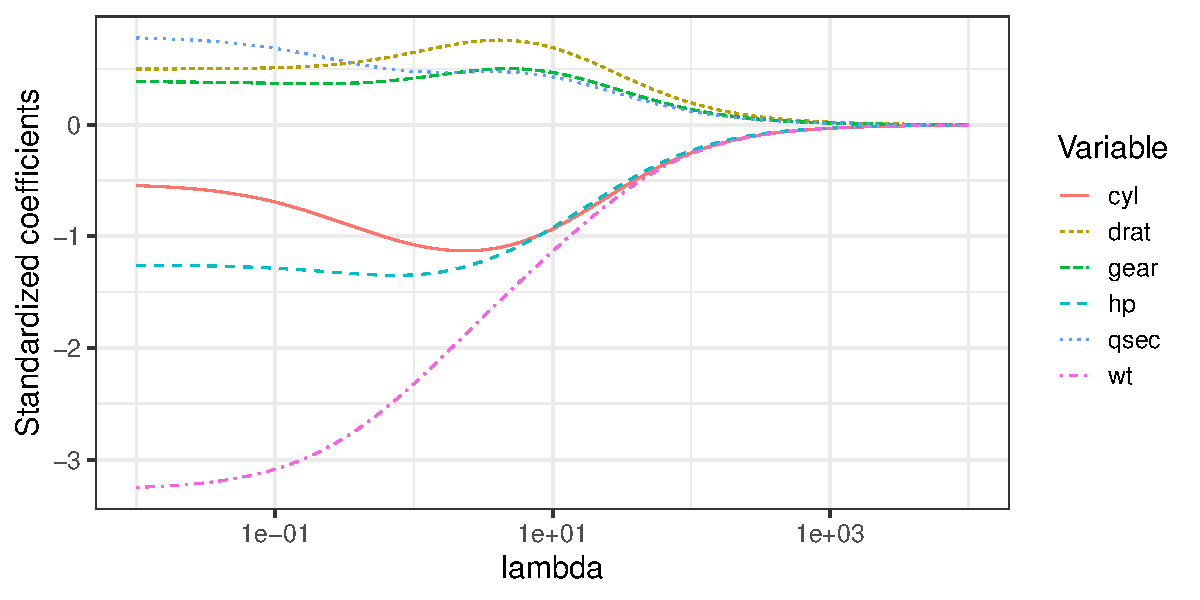
\includegraphics[width=.7\textwidth]{scripts/output/ridge_coefficient.pdf}
    \caption{The effect of $\lambda$ on coefficents in a ridge regression model for the \texttt{mtcars} dataset.}
  \end{figure}
\end{frame}

\begin{frame}{\secname}{\subsecname}
  A benefit of ridge regression is that it can be solved analytically, as the minimization problem is
  \begin{align}
    RSS(\lambda) = (\mathbb{Y} - \mathbb{X}\beta)^\top(\mathbb{Y} - \mathbb{X}\beta) - \lambda\beta^\top\beta.
  \end{align}
  If we the above function be the lagrange function, differentiate w.r.t.\! $\beta$ and set this equal to zero we find that
  \begin{align}
    \hat{\beta}^R = (\mathbb{X}^\top\mathbb{X} + \lambda I)^{-1}\mathbb{X}^\top\mathbb{Y}.
  \end{align}
  It is easy to compute as it is just a closed form expression and we can again observe that for $\lambda = 0$ we get the OLS estimate.
\end{frame}

\subsection{Lasso}
\begin{frame}{\secname}{\subsecname}
  The expression that lasso looks to minimize is the following
  \begin{align*}
    \sum_{i=1}^n \left(y_i - \beta_0 - \sum_{j=1}^p \beta_j x_{ij}\right)^2 + \lambda \sum_{j=1}^p |\beta_j|, 
  \end{align*}
  where $\lambda$, again, is a parameter that needs to be determined seperately.

  As opposed to ridge regression, lasso can force coefficients to exactly zero and thereby perform variable selection.
\end{frame}

\begin{frame}{\secname}{\subsecname}
  \begin{figure}
    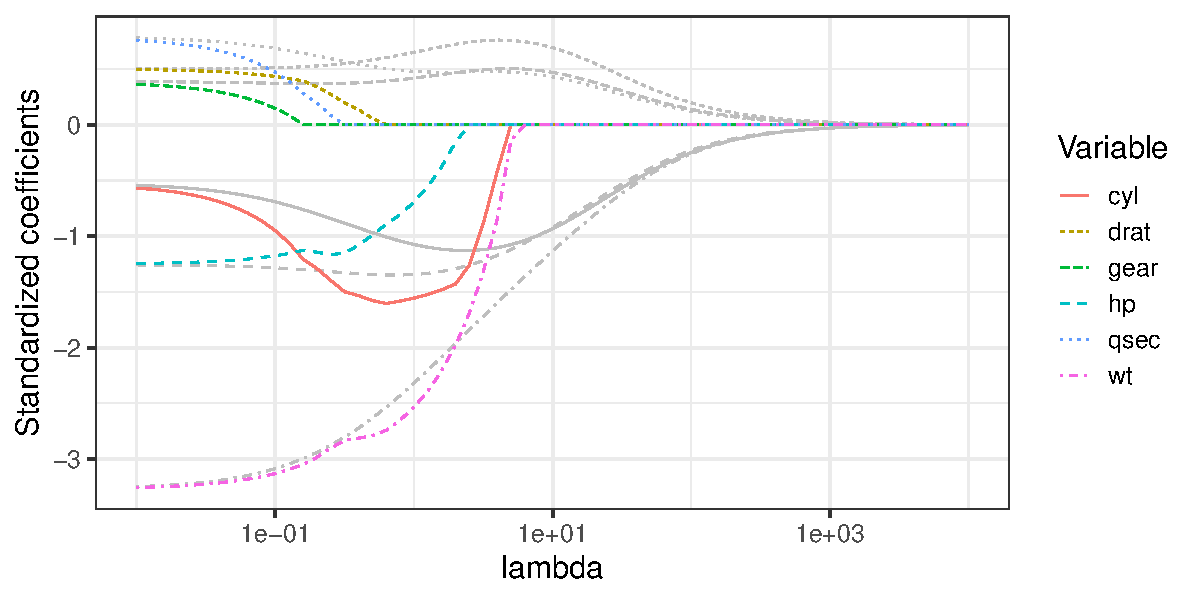
\includegraphics[width=.7\textwidth]{scripts/output/lasso_coefficient.pdf}
    \caption{The effect of $\lambda$ on coefficents in a lasso regression model for the \texttt{mtcars} dataset.
    Ridge coefficients are included as gray lines for reference.}
  \end{figure}
\end{frame}

\begin{frame}{\secname}{\subsecname}
  Unlike ridge regression, there does not exists an analytical solution for the lasso estimates.
  This is because the absolute value is \textbf{not} differentiable.
  
  Therefore we must resort to numerical optimization.

  For this we can use a method called \textbf{coordinate descent}, that works in the following way:

  Instead of trying to solve for all parameters at once we will look for a solution one dimension at a time.
  When we are done with one dimension we go to the next and then iterate through until we converge.
\end{frame}

\begin{frame}{\secname}{\subsecname}
  For the following computations we will assume that the data have been demeaned so we can disregard $\beta_0$.

  We then start the coordinate descent by the following minimization problem ({\color{orange}orange} term is just to simplify computation, $N$ is the number of observations and $p$ is the number of variables)
  \begin{align}
    \min_{\beta_j} \Bigg\{ {\color{orange}\dfrac{1}{2N}} \sum_{i=1}^N \left( y_i - \sum_{j=1}^p x_j \beta_j\right)^2 + \lambda \sum_{j=1}^p |\beta_j| \Bigg\}.
  \end{align}
  Let us define a function $L$ as
  \begin{align}
    L = \dfrac{1}{2N} \sum_{i=1}^N \left( y_i - \sum_{j=1}^p x_j \beta_j\right)^2 + \lambda \sum_{j=1}^p |\beta_j|
  \end{align}
\end{frame}

\begin{frame}{\secname}{\subsecname}
  If we then differentiate w.r.t.\! $\beta_k$ we get
  \begin{align}
    \frac{\partial L}{\partial \beta_k} &= N^{-1} \sum_{i=1}^N \left( y_i - \sum_{j=1}^p x_j \beta_j\right)\left(-x_k\right) + \lambda \underbrace{{\color{orange}\partial|\beta_k|}}_{Subgradient} \\
    &= N^{-1} \sum_{i=1}^N \left( y_i - \sum_{j\neq k}^p x_j \beta_j - x_k \beta_k\right)\left(-x_k\right) + \lambda \partial|\beta_k| \\
    &= N^{-1} \sum_{i=1}^N \left( {\color{violet}y_i - \sum_{j\neq k}^p x_j \beta_j}\right)\left(-x_k\right) + N^{-1}\beta_k\sum_{i=1}^N x_k^2 + \lambda \partial|\beta_k|
  \end{align}
  We can define the purple term as $r_k = y_i - \sum_{j\neq k}^p x_j \beta_j$ as this is the residual from the model w.o. the $k$'th regressor.
\end{frame}

\begin{frame}{\secname}{\subsecname}
  We can then write
  \begin{align}
    &=-N^{-1} \sum_{i=1}^N \left( r_k x_k\right) + N^{-1}\beta_k\sum_{i=1}^N x_k^2 + \lambda \partial|\beta_k| \\
    &=-N^{-1} r_k^\top x_k + N^{-1} x_k^\top x_k\beta_k + {\color{orange}\lambda \partial|\beta_k|},
  \end{align}
  So now we need to figure out what to do with the {\color{orange} subgradient}.
\end{frame}

\begin{frame}{\secname}{\subsecname}
  \begin{columns}
    \begin{column}{.7\textwidth}
      As there are lots of lines tangent to the absolute value in zero, we can summarize the subgradient as
      \begin{align}
        \lambda\partial|\beta_k| =
        \begin{cases}
          -\lambda &\text{if } \beta_k < 0 \\
          [-\lambda, \lambda] &\text{if } \beta_k = 0\\
          \lambda &\text{if } \beta_k > 0
        \end{cases},
      \end{align}
      for $\beta_k = 0$ the gradient can take all values between -1 and 1.
    \end{column}
    \begin{column}{.3\textwidth}      
      \begin{figure}
        \begin{subfigure}[t]{\textwidth}
          \centering
          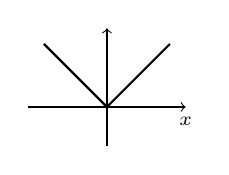
\begin{tikzpicture}
            \draw[->] (-1,0) -- (1,0);
            \draw[->] (0,-.5) -- (0,1);
            \node[anchor=north] at (1,0) {{\scriptsize $x$}};

            \draw[thick] (-.8,.8) -- (0,0) -- (.8,.8);
          \end{tikzpicture}
          \caption{$f(x) = |x|$.}
        \end{subfigure}
        \vfill
        \begin{subfigure}[t]{\textwidth}
          \centering
          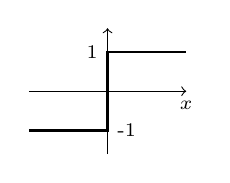
\begin{tikzpicture}
            \draw[->] (-1,0) -- (1,0);
            \draw[->] (0,-.8) -- (0,.8);
            \node[anchor=north] at (1,0) {{\scriptsize $x$}};

            \draw[thick] (-1,-.5) -- (0,-.5) -- (0,.5) -- (1,.5);
            \node[anchor=west] at (0,-.5) {{\scriptsize -1}};
            \node[anchor=east] at (0,.5) {{\scriptsize 1}};
          \end{tikzpicture}
          \caption{$\partial f(x)$.}
        \end{subfigure}
        \caption{The absolute value and its gradient.}
      \end{figure}
    \end{column}
  \end{columns}
\end{frame}

\begin{frame}{\secname}{\subsecname}
  This means that we can rewrite the derivative as the following
  \begin{align}
    \frac{\partial L}{\partial \beta_k} = 
    \begin{cases}
      -N^{-1} r_k^\top x_k + N^{-1} x_k^\top x_k\beta_k - \lambda &\text{if } \beta_k < 0 \\
      [-N^{-1} r_k^\top x_k - \lambda, -N^{-1} r_k^\top x_k + \lambda] &\text{if } \beta_k = 0 \\
      -N^{-1} r_k^\top x_k + N^{-1} x_k^\top x_k\beta_k + \lambda &\text{if } \beta_k > 0
    \end{cases}.
  \end{align}
  Setting this equal to zero and solving for $\beta_k$ in the 3 cases gives us the estimates, we take the case $\beta_k < 0$ as an example
  \begin{align}
    \frac{\partial L}{\partial \beta_k} = 0 \Leftrightarrow -N^{-1} r_k^\top x_k + N^{-1} x_k^\top x_k\beta_k - \lambda &= 0 \\
    N^{-1} x_k^\top x_k\beta_k &= N^{-1} r_k^\top x_k + \lambda \\
    \beta_k &=\left(N^{-1} x_k^\top x_k\right)^{-1}\left({\color{orange} N^{-1} r_k^\top x_k + \lambda}\right).
  \end{align}
\end{frame}

\begin{frame}{\secname}{\subsecname}
  Note that
  \begin{align}
    \beta_k < 0 \quad \Leftrightarrow \quad N^{-1}r_k^\top x_k + \lambda < 0 \quad \Leftrightarrow \quad N^{-1}r_k^\top x_k < - \lambda. 
  \end{align}

  Ultimately we find that, these are the values to update parameters by
  \begin{align}
    \hat{\beta}_k =
    \begin{cases}
      \left(N^{-1} x_k^\top x_k\right)^{-1}\left( N^{-1} r_k^\top x_k + \lambda\right) &\text{if } N^{-1}r_k^\top x_k < -\lambda\\
      0 &\text{if } -\lambda \leq N^{-1}r_k^\top x_k \leq \lambda\\
      \left(N^{-1} x_k^\top x_k\right)^{-1}\left( N^{-1} r_k^\top x_k - \lambda\right) &\text{if } N^{-1}r_k^\top x_k > \lambda
    \end{cases},
  \end{align}
  and we remember that $r_k$ is the residual from the model w.o.\! the $k$'th regressor.
\end{frame}

\subsection{Elastic Net}
\begin{frame}{\secname}{\subsecname}
  The method is a compromise between Ridge Regression and Lasso as it minimizes
  \begin{align*}
    \sum_{i=1}^n \left( y_i - \beta_0 - \sum_{j=1}^p \beta_j x_{ij}\right)^2 + \lambda \sum_{j=1}^p \left(\alpha |\beta_j| + (1 - \alpha)\beta_j^2\right),
  \end{align*}
  note that here we have the additional parameter $\alpha$ that determines the weighting of the two norms.
\end{frame}

\begin{frame}{\secname}{\subsecname}
  \begin{columns}
    \begin{column}{.5\textwidth}
      \begin{itemize}
        \item The figure illustrates the feasible region, in the case of two variables, on the RSS surface.
        \item Most likely the OLS estimate will be somwhere outside the shapes plotted.
        \item A lasso estimate is more likely to be at the edges.
        \item Elastic net keeps the pointy edges but rounds the sides (depending on $\alpha$).
        \item Elastic net performs variable selection like the lasso, but shrinks correlated regressors like ridge.
      \end{itemize}
    \end{column}
    \begin{column}{.5\textwidth}
      \begin{figure}
        \centering
        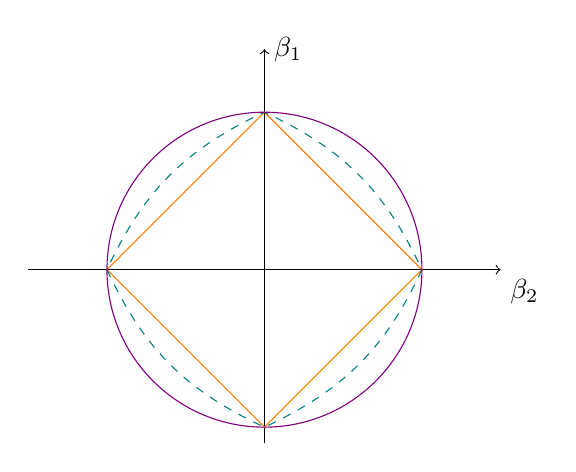
\begin{tikzpicture}
          \draw[->] (-3,0) -- (3,0);
          \node[anchor=west] at (0,2.8) {$\beta_1$};
          \draw[->] (0,-2.2) -- (0,2.8);
          \node[anchor=north west] at (3,0) {$\beta_2$};
          
          \draw[color=orange] (2,0) -- (0,-2) -- (-2,0) -- (0,2) -- (2,0);
          \draw[dashed, color=teal] (2,0) to [bend left=20] (0,-2) to [bend left=20] (-2,0) to [bend left=20] (0,2) to [bend left=20] (2,0);
          \draw[color=violet] (0,0) circle (2);
        \end{tikzpicture}
        \caption{The feasible region for {\color{orange} ridge}, {\color{violet} lasso} and {\color{teal} elastic net} ($\alpha = .5$).}
      \end{figure}
    \end{column}
  \end{columns}
\end{frame}

\subsection{Scaling of variables}
\begin{frame}{\secname}{\subsecname}
  For both shrinkage methods it is important to scale the variables before fitting the model.

  Contrary to linear regression where the scaling of variables are absorbed in the coefficients, this will affect the penalty term for both shrinkage methods.

  For example if a variable takes very large values it will get a higher penalty than a variable that takes small values, just because of the unit of measurement.
\end{frame}

\section{Classification}

\subsection{Introduction}
\begin{frame}{\secname}{\subsecname}
  If the response variable is categorical (qualitative), i.e.\! it is of the form $y\in\{1,\ldots,L\}$. Then a linear model of the form
  \begin{align*}
    y = \beta_0 + \beta_1 x_1 + \cdots + \beta_px_p,
  \end{align*}
  is generally not a good approach to take as it could predict invalid values and for certain types of categorical data there might not be a clear ordering.
  
  Therefore when dealing with categorical variable the aim of the model is to predict the probability that an observation belongs to a certain category, rather than the category itself.
\end{frame}

\subsection{Logistic Regression}
\begin{frame}{\secname}{\subsecname}
  To begin with let us assume the simple case that $y\in \{0,1\}$ and that we would like to model
  \begin{align}
    p(Y = 1 | X_i) = p(X_i) = \beta_0 + \beta_1 x_1 + \cdots + \beta_px_p = X_i \mathbb{B}.
  \end{align}
  Given that we know probabilities lie between 0 and 1, we would like to transform the linear function such that the output is between 0 and 1.

  The most popular, although there are several, would be the logistic function
  \begin{align}
    p(X_i) = \frac{e^{X_i \mathbb{B}}}{1 + e^{X_i \mathbb{B}}}.
  \end{align}
  For $X_i \beta \rightarrow \infty$ then $p(X_i) \rightarrow 1$ and for $X_i \beta \rightarrow - \infty$ then $p(X_i) \rightarrow 0$.
\end{frame}

\subsection{Linear Discriminant Analysis (LDA)}
\begin{frame}{\secname}{\subsecname}
  Suppose we have a dataset with a response variable $y\in\{0,\ldots,L\}$, explanatory variables $x_1, \ldots, x_p$ and that we would like to model
  \begin{align}
    P(y=k|X) =\underbrace{\frac{P(y = k)P(X|y=k)}{P(X)}}_{\text{Bayes Theorem}} = \frac{\pi_k f_k(x)}{\sum_{i=1}^K f_i(x)},
  \end{align}
  where $\pi_k = P(y=k)$ and $f_k(x) = P(X|y=k)$.

  If we use the proportion of observations in the dataset that belong to class $k$ as an estimate for $\pi_k$, then we just need to model $f_k(x) =P(X|y=k)$.

  In other words we need to make some assumption on the distribution of $f_k(x)$.
\end{frame}

\begin{frame}{\secname}{\subsecname}
  The assumption made in LDA is that each $f_k(x)$ come from a multivariate normal distribution, i.e.\!
  \begin{align}
    f_k(x) = \frac{1}{(2\pi)^{p/2} |\Sigma_k|^{1/2}} \exp\left\{
      -\frac{1}{2}(x - \mu_k)^\top\Sigma_k^{-1}(x - \mu_k)
    \right\}.
  \end{align}
  Another assumption made in LDA is that $\Sigma_k = \Sigma \ \forall k \in \{1,\ldots,K\}$, in other words all classes will have the same variance-covariance matrix.
\end{frame}

\begin{frame}{\secname}{\subsecname}
  When we classify a new observation, $X_0$, we simply find the category with the highest probability, $P(y = k|X_0)$ for $k = 1,\ldots,K$.

  In other words we want to find the $k$ such that $P(y=k|X)$ is maximized.
  Since the logarithm is an increasing function we know that the $k$ which maximizes $P(y=k|X)$ also maximizes the following
  \begin{align}
    \log(P(y=k|X)) = \log(\pi_k) + \log(f_k(x)) - \underbrace{\log\left(\sum_{i = 1}^K \pi_i f_i(x)\right)}_{\text{Does not depend on $k$}},
  \end{align} 
  The last term is identical across categories and we drop this term for the maximization problem.
\end{frame}

\begin{frame}{\secname}{\subsecname}
  So now we have the following
  \begin{align}
    \log(\pi_k) + \log(f_k(x)), \label{eq:lda_two_terms}
  \end{align}
  but let us take a look at the second term.
  By the normality assumption we have that
  \begin{align}
    f_k(x) = \frac{1}{(2\pi)^{p/2} |\Sigma|^{1/2}} \exp\left\{
      -\frac{1}{2}(x - \mu)^\top\Sigma^{-1}(x - \mu_k)
    \right\}.
  \end{align}
  Thus we can write \eqref{eq:lda_two_terms} as
  \begin{align}
    \log(\pi_k) + \underbrace{\log((2\pi)^{p/2} |\Sigma|^{1/2})}_{\text{Does not depend on $k$}} - \frac{1}{2}(x - \mu)^\top\Sigma^{-1}(x - \mu_k), 
  \end{align}
  and subsequently drop another term that is identical across categories.
\end{frame}

\begin{frame}{\secname}{\subsecname}
  So now we have the following
  \begin{align}
    \log(\pi_k) - \frac{1}{2}(x - \mu)^\top\Sigma^{-1}(x - \mu_k), \label{eq:lda_another_two_terms}
  \end{align}
  again taking a look at the second term
  \begin{align}
    (x - \mu_k)^\top\Sigma^{-1}(x - \mu_k) = \underbrace{x^\top\Sigma^{-1}x}_{\text{Does not depend on $k$}} - x^\top\Sigma^{-1}\mu_k - \mu_k^\top \Sigma^{-1}x + \mu_k^\top \Sigma^{-1}\mu_k, 
  \end{align}
  and furthermore we have that $x^\top\Sigma^{-1}\mu_k = \mu_k^\top \Sigma^{-1}x$ because both are scalars and one is just the transpose of the other.
\end{frame}

\begin{frame}{\secname}{\subsecname}
  So we end up with the following expression, which is called the \textbf{linear discriminant function}
  \begin{align}
    \delta_k(x) = \log(\pi_k) + x^\top \Sigma^-1 \mu_k - \frac{1}{2}\mu_k^\top \Sigma^{-1} \mu_k,
  \end{align}
  this is what we will use to classify observations.
  Note the expression is linear in $x$ and therefore we call it linear discriminant analysis.
\end{frame}

\begin{frame}{\secname}{\subsecname}
  In practice the parameters are estimated by
  \begin{align}
    \hat{\pi}_k = \frac{n_k}{n}, \quad \hat{\mu}_k = \frac{1}{n_k}\sum_{y_i=k}x_i, \quad \hat{\Sigma} \frac{1}{n-K}\sum_{k=1}^K\sum_{y_i=k}(x_i - \hat{\mu}_k)(x_i - \hat{\mu}_k)^\top,
  \end{align}
  i.e.\! the proportion of observations in class $k$, the mean for class $k$ and the mean of the variances respectively.
\end{frame}

\subsection{Quadratic Discriminant Analysis (QDA)}
\begin{frame}{\secname}{\subsecname}
  Imagine now that we relax the LDA assumption that $\Sigma_k = \Sigma \ \forall k \in \{1,\ldots,K\}$ and allow classes to have their own variance-covariance matrix.

  This implies that some of the simplification we performed before no longer holds and the discriminant function will now take the form
  \begin{align}
    \delta_k(x) = {\color{orange}-\frac{1}{2} x^\top\Sigma_kx} + \log(\pi_k) + x^\top \Sigma{\color{orange}_k}^-1 \mu_k - \frac{1}{2}\mu_k^\top \Sigma{\color{orange}_k}^{-1} \mu_k {\color{orange}- \frac{1}{2}\log|\Sigma_k|},
  \end{align}
  note that first term is quadratic in $x$.

  Another difference in the estimation of the covariance matrices, because we relaxed the assumption we must estimate a variance-covariance matrix for each class
  \begin{align}
    \hat{\Sigma}_k = \frac{1}{n_k - 1} \sum_{y_i = k} (x_i - \hat{\mu}_k)(x_i - \hat{\mu}_k)^\top.
  \end{align}
\end{frame}

\subsection{Example using the Iris dataset}
\begin{frame}{\secname}{\subsecname}
  \begin{figure}
    \centering
    \begin{subfigure}[b]{0.45\textwidth}
      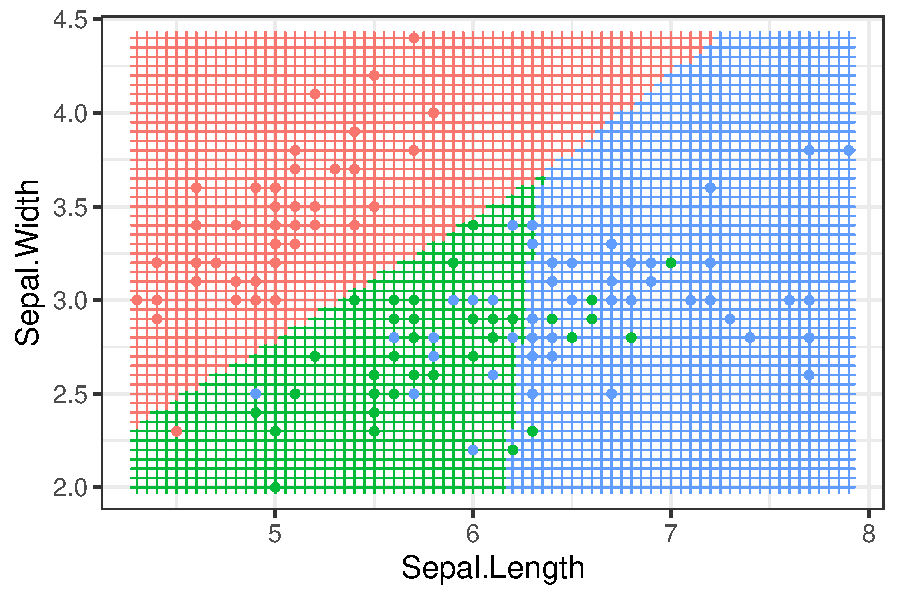
\includegraphics[width=\textwidth]{scripts/output/lda_regions.pdf}
      \caption{LDA classification regions.}
    \end{subfigure}
    \hfill
    \begin{subfigure}[b]{0.45\textwidth}
      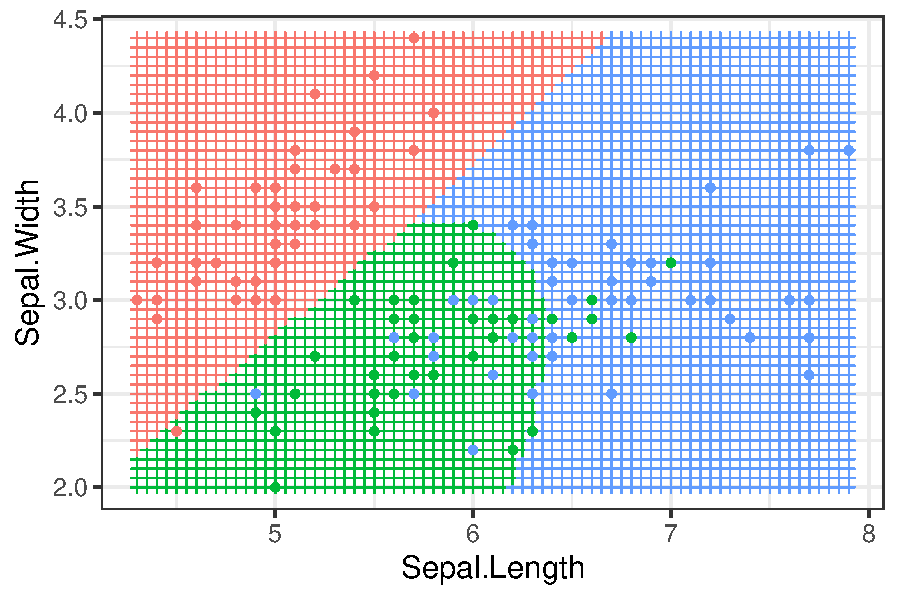
\includegraphics[width=\textwidth]{scripts/output/qda_regions.pdf}
      \caption{QDA classification regions.}
    \end{subfigure}
    \caption{Classification regions for LDA and QDA performed on the \textit{Iris} dataset, considering only the variables \textit{sepal width} and \textit{sepal length}.
    Note that the LDA boundaries are linear while QDA include a non-linear boundary.}
  \end{figure}
\end{frame}

\subsection{Example using Auto dataset}
\begin{frame}{\secname}{\subsecname}
  \begin{figure}
    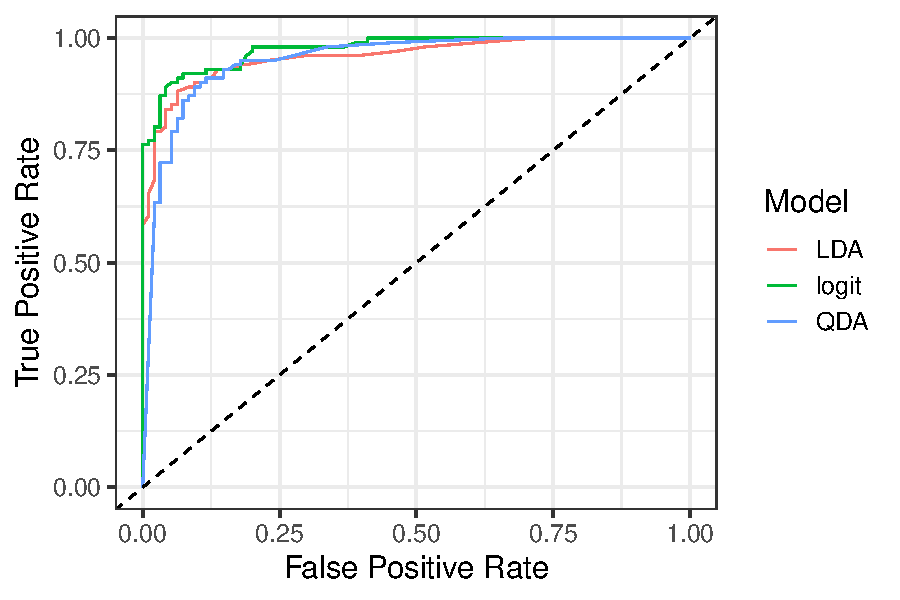
\includegraphics[width=.55\textwidth]{scripts/output/mpg_roc.pdf}
    \caption{ROC curves for 3 models on the \textit{auto} dataset from the \texttt{ISLR} package. We are predicting whether a car have mpg above the median using displacement, weight, year and horsepower.}
  \end{figure}
\end{frame}

\subsection{Naive Bayes}
\begin{frame}{\secname}{\subsecname}
  The (Naive) Bayes classifier is an example of a parametric classifier (meaning that the number of parameters is fixed), it builds on Bayes theorem
  \begin{align}
    P(Y = i| X) = \frac{P(Y = i)P(X| Y=i)}{P(X)}.
  \end{align}
  New data is then assigned to the class with the highest probability given the explanatory variables
  \begin{align}
    \hat{Y} = \textit{ arg max}_i P(Y = i)P(X | Y = i).
  \end{align}
  This means that there are two things we need to model, the first is $P(Y = i)$, but this is simply modelled by the proportions of the dataset.
\end{frame}

\begin{frame}{\secname}{\subsecname}
  The second one is $P(X | Y = i)$, note that $X$ is a $p$-dimensional vector, making the distribution multivariate.
  
  However as estimating multivariate distribution requires lots of computation and suffers from the curse of dimensionality, an assumption in Naive Bayes is that $X$ is independent between classes
  \begin{align}
    P(X | Y_i) = P(X_1|Y)P(X_2|Y)\cdots P(X_p|Y).
  \end{align}
  With this assumption we can rewrite
  \begin{align}
    P(X | Y = i) = \prod_{j=1}^p P(X_j | Y = i),
  \end{align}
  which enables us to estimate all marginal (univariate) distributions one by one.
\end{frame}

\begin{frame}{\secname}{\subsecname}
  Typically the we assume that the ditributions are normal, but we can also use others and even seperate distributions for each explanatory variable.

  In the case of normally distributed variables we only need to estimate the mean and variance as $X_j | Y = i \sim N(\mu_{j,i}, \sigma^2_{j,i})$, where we use the usual estimates
  \begin{align}
    \mu_{j,i} = \frac{1}{N_i} \sum_{x_k | y_k = i} x_{j,i}, \quad
    \sigma_{j,i}^2 = \frac{1}{N_i} \sum_{x_k | y_k = i}(x_{j,i} - \mu_{j,i})^2.
  \end{align}
  Despite the assumption of independence the method tends to work well in practice, although if the assumption is clearly not true we will get biased estimator.
\end{frame}

\section{Trees}

\subsection{Introduction}
\begin{frame}{\secname}{\subsecname}
  Tree-based methods are supervised learning methods which can be used for both regression and classification.
  
  They work by segmenting the space into a number of simple regions and then, typically, use the mean of the region to make predictions.
  
  Because the segmentation of the space can be summarized in a tree, we call these methods tree-based.
\end{frame}

\subsection{Classification and Regression Trees (CART)}
\begin{frame}{\secname}{\subsecname}
  The purpose of the CART algorithm is to decide on the split points. This is done in a greedy way one split at a time, as the task of checking all possible combinations of splits would be computationally infeasible.

  We look for split points by solving (here we assume that the loss function in the $\ell_2$ norm)
  {\small\begin{align*}
      \min_s \left[\min_{c_1} \sum_{x_i < s} \left(y_i - c_1\right)^2 + \min_{c_2} \sum_{x_i \geq s}\left(y_i - c_2\right)^2\right],  
  \end{align*}}
  so we wish to find a split point $s$ that minimizes the loss function on either side. 
  Recall that {\small $$\Tilde{y}_1 = min_{c_1} \sum_{x_i < s} (y_i - c_1)^2 \text{ and } \Tilde{y}_2 = min_{c_2} \sum_{x_i \geq s} (y_i - c_2)^2.$$} 
  Where $\Tilde{y}_1$, $\Tilde{y}_2$ are the means for $y_i$ such that $x_i < s$ and $x_i \geq s$ respectively.
\end{frame}

\begin{frame}{\secname}{\subsecname}
  The split points we find produces basis functions $b_1(x) = I(x_i < s)$ and $b_2(x) = I(x_i \geq s)$, which would be equivalent to fitting the model
  \begin{align}
      y_i = \beta_1 b_1 (x_i) + \beta_2 b_2 (x_i).
  \end{align}
  Next step is to repeat the same procedure in the new regions, that is we find the best split points in each of the new regions and the choose the best.

  We do this until hit some predetermined stopping criteria, could be minimum number of observations in each region, not enough increase in fit etc.
\end{frame}

\begin{frame}{\secname}{\subsecname}
  \begin{figure}
    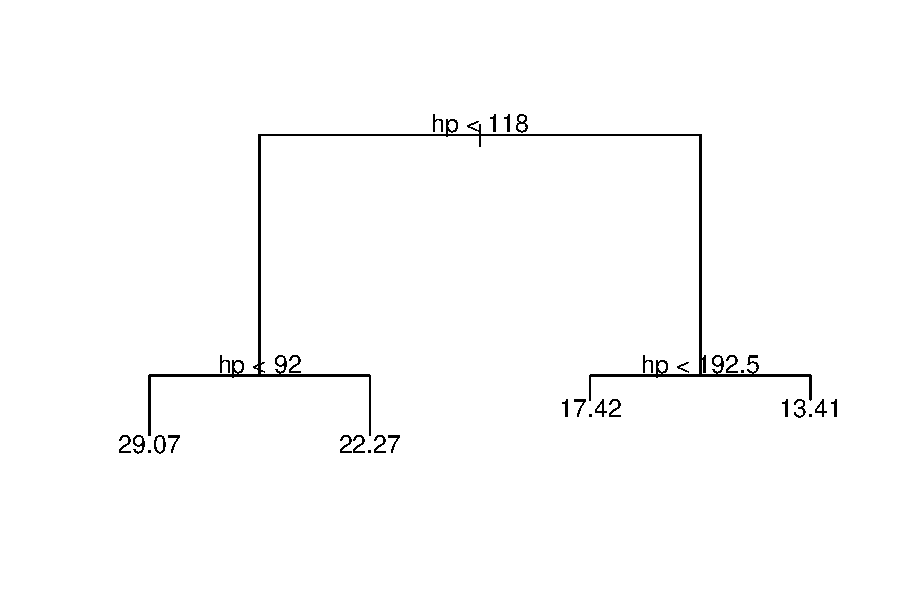
\includegraphics[width=.6\textwidth]{scripts/output/uni-tree.pdf}
    \caption{A decision tree explaining \textit{miles per gallon} by \textit{horsepower}.}
  \end{figure}
\end{frame}

\begin{frame}{\secname}{\subsecname}
  For the univariate case it is pretty straigth forward, but what if we have more variables?

  It is still pretty straightforward, so the idea is to obtain possible cuts for each variable and the choose the best.
  Then we get two regions and we repeat the same procedure in each.
  This method is called \textbf{recursive binary splitting}.

  Formally this can be expressed as, first defining regions
  {\small\begin{align}
    R_1 (j,s) = \{ X | X_j < s \}, \quad
    R_2 (j,s) = \{X | X_j \geq s\},
  \end{align}}
  then finding the cutpoint amounts to solving
  {\small\begin{align}
    \min_{j,s} \left[ \sum_{ \{ i | x_i \in R_1 (j,s)\} } (y_i - \tilde{y}_{R_1})^2 + \sum_{\{ i | x_i \in R_2(j,s) \}} (y_i - \tilde{y}_{R_2})^2\right].
  \end{align}}
\end{frame}

\begin{frame}{\secname}{\subsecname}
  \begin{figure}
    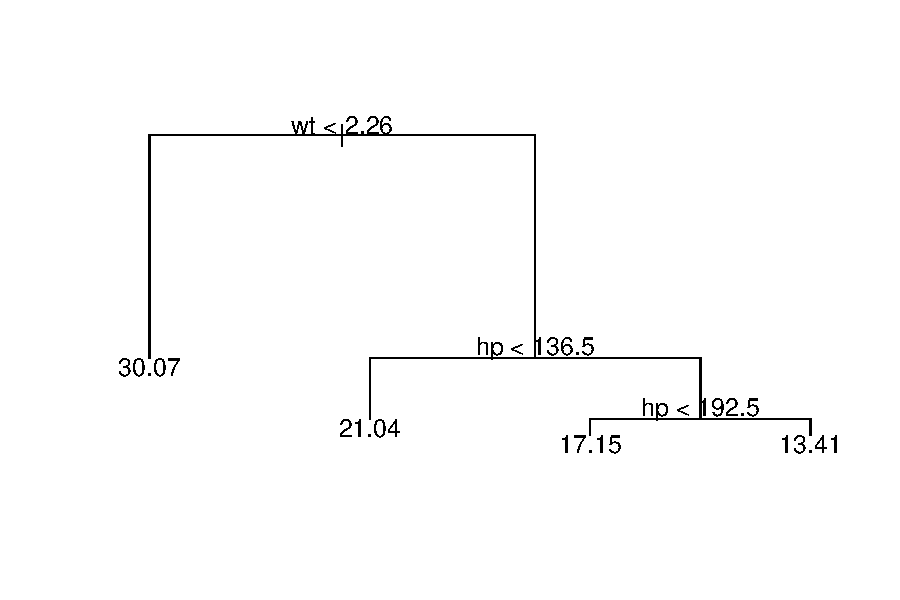
\includegraphics[width=.6\textwidth]{scripts/output/multi-tree.pdf}
    \caption{A decision tree explaining \textit{miles per gallon} by \textit{horsepower} and \textit{weight}.}
  \end{figure}
\end{frame}

\subsection{Pruning}
\begin{frame}{\secname}{\subsecname}
  A
\end{frame}

\subsection{Comparing Linear Regression and CART}

\begin{frame}{\secname}{\subsecname}
  \begin{columns}
    \begin{column}{.5\textwidth}
      \begin{itemize}
        \item So how do CART compare to linear regression?
        \item Well it depends on the data.
      \end{itemize}
    \end{column}
    \begin{column}{.5\textwidth}
      \begin{figure}
        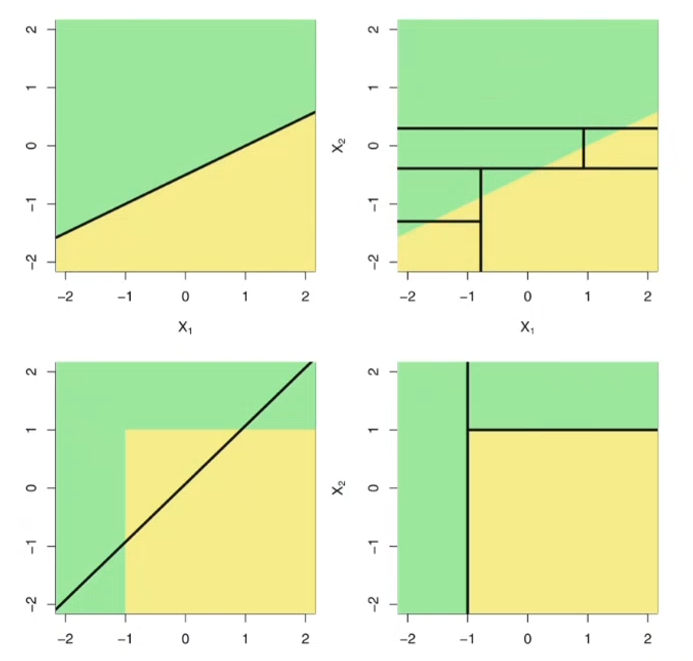
\includegraphics[width=.9\textwidth]{scripts/output/types-of-data.png}
      \end{figure}
    \end{column}
  \end{columns}
\end{frame}

\begin{frame}{\secname}{\subsecname}
  Consider the following model (non-binary)
  \begin{align}
    y = 1 + 2x_1 + 3x_2 + \varepsilon,
  \end{align}
  where $x_1, x_2 \sim N(0,1)$ and $\varepsilon \sim N(0,1/2)$.
  We can then introduce the variables $\tilde{x}_1, \tilde{x}_2$ given by
  \begin{align}
    \tilde{x}_1 =
    \begin{cases}
      1 & \text{for } x_1 > 0 \\
      0 & \text{for } x_1 \leq 0
    \end{cases},
    \quad
    \tilde{x}_2 =
    \begin{cases}
      1 & \text{for } x_2 > 0 \\
      0 & \text{for } x_2 \leq 0
    \end{cases},
  \end{align} 
  and proprose a separate model (binary)
  \begin{align}
    \tilde{y} = 1 + 2\tilde{x}_1 + 3\tilde{x}_2 + \varepsilon.
  \end{align}
  We can then compare how the CART algorithm compares to linear regression on both the binary and non-binary model.
\end{frame}

\begin{frame}{\secname}{\subsecname}
  \begin{figure}
    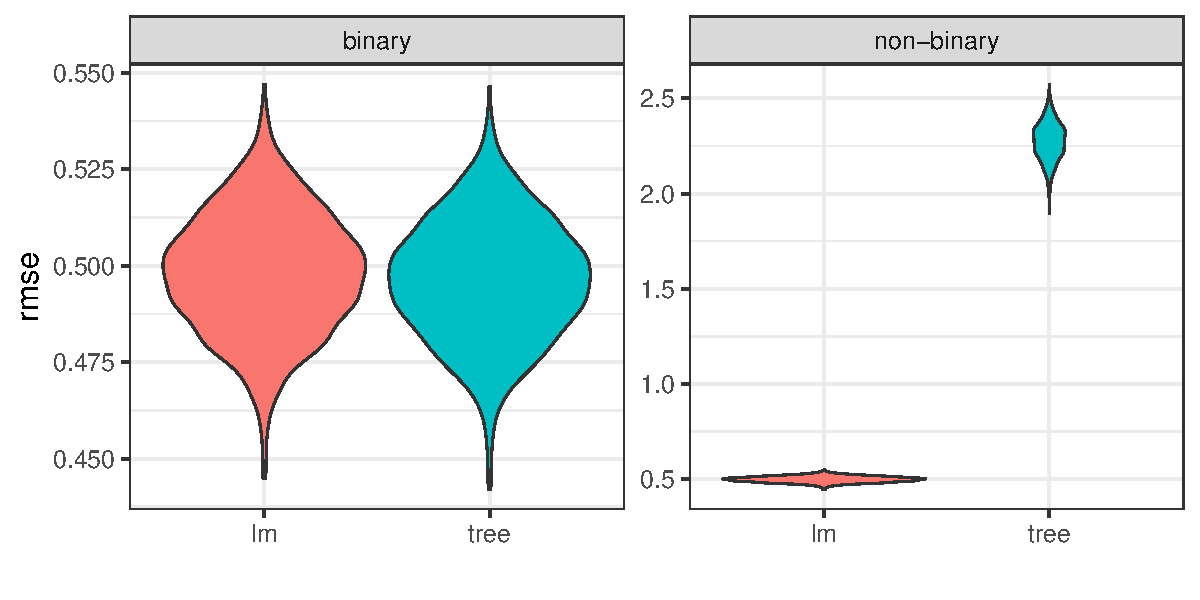
\includegraphics[height=.5\textheight]{scripts/output/lm_tree_compare.pdf}
    \caption{Comparing linear regression (\texttt{lm} from \texttt{base R}) and CART (\texttt{tree} from the \texttt{tree} package) on 1000 repetions of 500 observations.
    We see that when the data is generated from a step function its a tie between \texttt{tree} and \texttt{lm}, but when the data is linear the CART understandably struggles compared to linear regression.}
  \end{figure}
\end{frame}

\subsection{Bagging}
\begin{frame}{\secname}{\subsecname}

\end{frame}

\subsection{Random Forest}
\begin{frame}{\secname}{\subsecname}

\end{frame}

\subsection{Boosting}
\begin{frame}{\secname}{\subsecname}

\end{frame}

\section{Support Vector Machines}

\subsection{Overview}
\begin{frame}{\secname}{\subsecname}
  
\end{frame}

\section{Neural Networks}

\subsection{Overview}
\begin{frame}{\secname}{\subsecname}
  
\end{frame}

\subsection{Perceptron}
\begin{frame}{\secname}{\subsecname}
    \textbf{Backpropagation}: For a given loss function $L$ we look for $\frac{\partial L}{\partial w_i}$.
    We start with initial values for the weights, which we shall denote $w_{old}$.
    Then we update the weights by $w_{new} = w_{old} - \eta \frac{\partial L}{\partial w}$.
    One iteration is called an \textbf{epoch}.
\end{frame}

{\aauwavesbg
\begin{frame}[plain,noframenumbering]
\end{frame}}
%%%%%%%%%%%%%%%%

\end{document}
